\documentclass[10pt, letterpaper]{article}
\usepackage{setspace}
\usepackage[letterpaper, margin=1.0in]{geometry}
\addtolength{\topmargin}{-0.25in}
%\usepackage{tocloft}
\usepackage{titlesec}
%\titleformat*{\section}{\large\bfseries}
\titleformat*{\section}{\large}
\titleformat*{\subsection}{\normalsize}
\usepackage{float}
\usepackage{longtable}
\usepackage{enumitem}
\usepackage{listings}
\usepackage{hyperref}
\hypersetup{colorlinks=true, urlcolor=blue}
\usepackage{amsmath}   % includes \boldmath(), \boldsymbol{()}
\usepackage{bm}        % math fonts, \boldmath{}, \boldsymbol{}
\usepackage{graphicx}
\graphicspath{{images/}}
\usepackage{subcaption}
\usepackage{xcolor, colortbl}
\definecolor{gray}{gray}{0.9}
\definecolor{ltBlue}{rgb}{0.75, 0.85, 0.975}
\definecolor{medBlue}{rgb}{0.75, 0.8, 0.9}
\definecolor{white}{rgb}{1, 1, 1}
\definecolor{midgreen}{rgb}{0.0, 0.5, 0.0}
%\rowcolor{ltBlue}
\usepackage{changepage}
\usepackage{pdflscape}
\bibliographystyle{plainnat}
\usepackage[authoryear, round, semicolon]{natbib}
\newcommand{\mt}[1]{\bm{#1}^{\prime}}
\newcommand{\mtm}[2]{\bm{#1}^{\prime}\bm{#2}}
\newcommand{\mi}[1]{\bm{#1}^{-1}}
\newcommand{\mest}[1]{\hat{\bm{#1}}}
\usepackage[bottom]{footmisc}
\setlength{\skip\footins}{12pt}
\setlength\parindent{0pt}

\title{\large \vspace{-0.5in} Duke University Circuit Court Appeals Project\\[10pt]
       Server and Database Connection Instructions\\[10pt] v 1.0, \today\\[-20pt]}

\date{}

\begin{document}

\begin{spacing}{1.0}
    
\maketitle

\section{Duke VPN Connection}

\begin{itemize}
    \item A Duke net ID is required.  Contact your colleague at Duke if you do not have one.
    \item Multifactor authentication (MFA) is required to access the Duke VPN.  You can configure an MFA device at \url{https://oit.duke.edu/what-we-do/applications/multi-factor-authentication}
    \item Download the Cisco VPN client from \url{https://oit.duke.edu/what-we-do/services/vpn}
    \item Connect to the Duke VPN through the VPN client:\\
    \begin{figure}[H]
        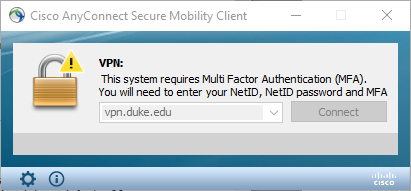
\includegraphics[width=2.9in]{VPN01.png}
        \centering
        \caption*{}
        \label{}
    \end{figure}
    \vspace{-0.45in}
    \begin{figure}[H]
        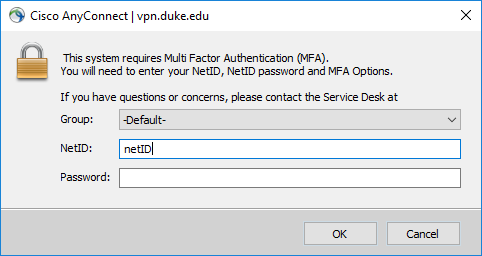
\includegraphics[width=2.9in]{VPN02.png}
        \centering
        \caption*{}
        \label{}
    \end{figure}
    \vspace{-0.45in}
    \begin{figure}[H]
        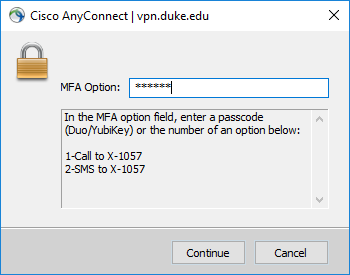
\includegraphics[width=2.9in]{VPN03.png}
        \centering
        \caption*{}
        \label{}
    \end{figure}  
\end{itemize}

\newpage

\section{Accessing the Appeals Data Server}\vspace{-2pt}

An SSH connection is required with port 3306 forwarded to the Appeals database server (MySQL communicates on port 3306 and requests from your local client will be forwarded to the server)

\begin{itemize}

    \item Unix, Mac, and Windows 10:  from the command line, open an ssh session with\\[2pt] \texttt{ssh -L 3306:127.0.0.1:3306 {\color{midgreen}netID}@lexnex-smben-01.oit.duke.edu}\\[2pt] where \texttt{{\color{midgreen}netID}} is your Duke net ID
    \item Windows pre-10\vspace{-0.02in}
      \begin{itemize}
          \item Download and install PuTTY from \url{https://www.chiark.greenend.org.uk/~sgtatham/putty/latest.html}
          \item From within PuTTY, create and name a connection to \texttt{lexnex-smben-01.oit.duke.edu} (complete highlighted fields):\\[-4pt]
          \begin{figure}[H]
              \includegraphics[width=3in]{Putty01.png}
              \centering
              \caption*{\vspace{-0.5in}}
              \label{}
          \end{figure}
          \vspace{-0.2in}
          \item On the SSH, Tunnels form, configure a port:\\[-4pt]
          \begin{figure}[H]
              \includegraphics[width=3in]{Putty02.png}
              \centering
              \caption*{\vspace{-0.5in}}
              \label{}
          \end{figure}
          \item Save, then open the connection:
          \begin{figure}[H]
              \includegraphics[width=3in]{Putty03.png}
              \centering
              \caption*{\vspace{-0.5in}}
              \label{}
          \end{figure}  
      \end{itemize}
    \item From ssh or PuTTY, open a session to the server.  You will be prompted for your Duke net ID, password, and an MFA method:\\
    \begin{figure}[H]
        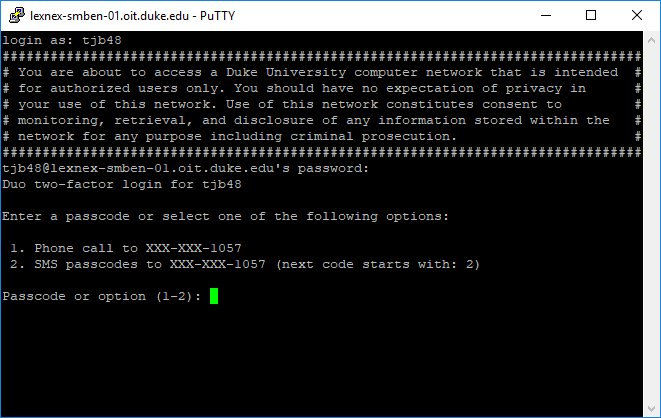
\includegraphics[width=4in]{ssh01.png}
        \centering
        \caption*{\vspace{-0.5in}}
        \label{}
    \end{figure}
    \newpage 
    \item Once you are authenticated, you will see the Unix prompt:\\
    \begin{figure}[H]
        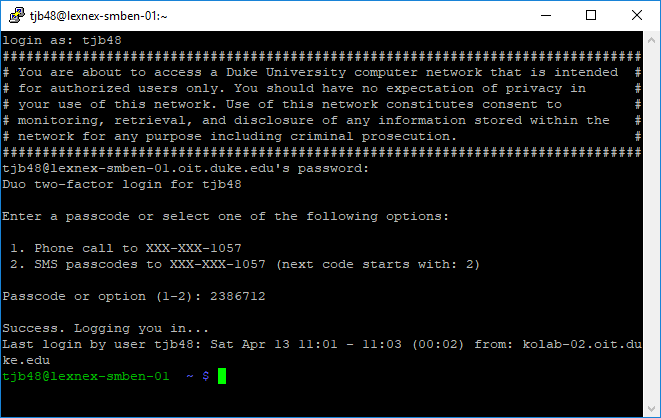
\includegraphics[width=4in]{ssh02.png}
        \centering
        \caption*{\vspace{-0.5in}}
        \label{}
    \end{figure}
    \item Port forwarding for MySQL to the DB server is now enabled.  Minimize the ssh window, but remember that you have an open connection to the server.  Be sure to close it when you no longer need access to the project database.
\end{itemize}

\section{Executing queries from within Rstudio}

\begin{itemize}

    \item Get database password from \href{mailto:thomas.balmat@duke.edu}{thomas.balmat@duke.edu}

    \item In the Rstudio console, install a few libraries that are needed for executing and testing queries:
    \small
    \begin{verbatim}
            install.packages("DBI")
            install.packages("RMySQL")
            install.packages("rstudioapi")
            install.packages("ggplot2")
            install.packages("xtable")
    \end{verbatim}
    \normalsize
    The above commands should be executed once only per computer.  Libraries become permanently available once installed.
    \newpage

    \item In the R console, set options, load libraries, and connect to the database (change NETID to your ID):
    \small
    \begin{verbatim}
            options(max.print=1000)      # number of elements, not rows
            options(stringsAsFactors=F)
            options(scipen=999999)
            options(device="windows")
            
            library(ggplot2)
            library(xtable)
            library(DBI)
            library(RMySQL)
            
            # Connect to Appeals database (prompt if in Rstudio)
            if(substring(R.Version()[["os"]], 1, 5)=="mingw") {
              db <- dbConnect(MySQL(), host="localhost", port=3306, dbname="Appeals",
              user="NETID",
              password=rstudioapi::askForPassword("Password:  "))
            } else {
              # Local connection
              db <- dbConnect(MySQL(), host="localhost", port=3306, dbname="Appeals",
                              user="NETID", password="")
            }
    \end{verbatim}
    \normalsize
    Enter your database password:\\
    \begin{figure}[H]
        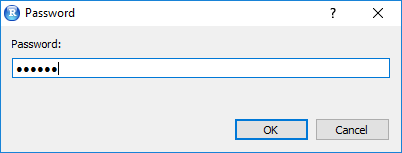
\includegraphics[width=3in]{DBPasswordPrompt.png}
        \centering
        \caption*{\vspace{-0.5in}}
        \label{}
    \end{figure}
    \vspace{-8pt}
    and verify that no error message appears in the R console

    \item You now have an active database connection.  List available tables:
    \small
    \begin{verbatim}
            dbGetQuery(db, "show tables")
    \end{verbatim}
    \normalsize
    \vspace{-8pt}
    Result:
    \small
    \begin{verbatim}    
               Tables_in_Appeals
            1         CaseHeader
            2       CaseLNTopics
            3    CaseLegalTopics
            4    CaseOutcomeType
            5           CaseType
            6  CaseTypeComposite
            7           Citation
            8              Court
            9          ImportRec
            10             Judge
            11           Opinion
            12             Panel
            13  ShepardTreatment
    \end{verbatim}
    \normalsize
    \newpage

    \item Aggregate cases by type and year:
    \scriptsize
    \begin{verbatim}
            # Aggregate cases by year and type
            # R warnings may be generated here
            # They can be suppressed with suppressWarnings(), but then all warnings are concealed

            sql <- "select   year(DecisionDate) as year, count(1) as n,
                             sum(case when(b.nCriminal=0 and nCivil>0)then 1 else 0 end) as nCivil,
                             sum(case when(b.nCriminal>0 and nCivil=0)then 1 else 0 end) as nCriminal,
                             sum(case when(b.nCriminal>0 and b.nCivil>0)then 1 else 0 end) as nCrimCiv,
                             sum(case when(b.LNI is null)then 1 else 0 end) as nNone
                    from     CaseHeader a
                             left join (select   LNI,
                                                 sum(case when(CaseType='Criminal')then 1 else 0 end) as nCriminal,
                                                 sum(case when(CaseType='Civil')then 1 else 0 end) as nCivil
                                        from     CaseType
                                        group by LNI) b on a.LNI=b.LNI
                    group by year(DecisionDate)"

            x <- dbGetQuery(db, sql)
                    
            print(x)
            
    \end{verbatim}
    \normalsize
    \vspace{-8pt}
    Result:
    \small
    \begin{verbatim}    
               year     n nCivil nCriminal nCrimCiv nNone
            1    NA    29      1         0        4    24
            2  1974  5406   1271       167     2638  1330
            3  1975  5621   1321       159     2867  1274
            4  1976  5618   1261       146     2973  1238
            5  1977  5398   1287       144     2863  1104
            6  1978  6604   1292       128     3159  2025
            7  1979  8772   1484       149     3218  3921
            8  1980 10829   1960       125     3764  4980
            9  1981 10626   1967       123     4162  4374
            10 1982 11201   1746        90     4807  4558
            11 1983 12208   2231        64     5323  4590
            12 1984 13411   2381        71     5533  5426
            13 1985 13784   2372        66     5860  5486
            14 1986 18736   2874        88     6213  9561
            15 1987 19594   3040       136     6139 10279
            16 1988 21560   3449       239     6235 11637
            17 1989 23392   3427       199     6328 13438
            18 1990 25901   3275       148     7599 14879
            19 1991 31364   4605       125    10160 16474
            20 1992 34692   4809       133    11281 18469
            21 1993 38117   4956       131    12011 21019
            22 1994 41913   6256       129    11934 23594
            23 1995 43150   5067       212    11248 26623
            24 1996 44659   4700       170    11738 28051
            25 1997 40697   4080       205    11332 25080
            26 1998 39323   4279       232    10774 24038
            27 1999 40441   5124       309    11533 23475
            28 2000 39921   5061       318    10925 23617
            29 2001 31387   4480       283    10503 16121
            30 2002 29578   4734       280    10991 13573
            31 2003 29185   4638       261    11571 12715
            32 2004 27379   4054       251    12189 10885
            33 2005 29025   4691       205    14801  9328
            34 2006 31847   5380       356    17079  9032
            35 2007 30391   8177       144    15963  6107
            36 2008 28153   7310       118    16153  4572
            37 2009 29571   9189       126    15776  4480
            38 2010 27567   9384       122    14483  3578
    \end{verbatim}
    \normalsize
    \vspace{-8pt}

    \item Plot distribution of cases by type and year (using x, from above):
    \scriptsize
    \begin{verbatim}
        # Sum cases by type
        y <- apply(as.matrix(c("n", "nCivil", "nCriminal", "nCrimCiv", "nNone")), 1, function(a) sum(x[,a]))
        sum(y[2:5])
        
        #dev.new()
        y <- data.frame("year"=x[,"year"],
        "type"=c(rep("criminal", nrow(x)), rep("civil", nrow(x)), rep("crim-civ", nrow(x)), rep("none", nrow(x))),
        "n"=c(x[,"nCriminal"], x[,"nCivil"], x[,"nCrimCiv"], x[,"nNone"]))
        
        ggplot() +
        geom_area(data=y, aes(x=year, y=n, fill=type), position="stack", alpha=0.75) +
        scale_fill_manual(name="", values=c("none"="blue2", "criminal"="orange2", "civil"="yellow3", "crim-civ"="purple2")) +
        scale_x_continuous(breaks=seq(1974, 2018, 4)) +
        scale_y_continuous(label=function(x) format(x, big.mark=",")) +
        labs(x="\nyear", y="cases\n") +
        theme(plot.title=element_text(size=12, hjust=0.5),
        plot.subtitle=element_text(size=10, hjust=0.5),
        plot.caption=element_text(size=10, hjust=0.5),
        panel.background=element_blank(),
        panel.grid.major.x=element_blank(),
        panel.grid.major.y=element_blank(),
        panel.grid.minor=element_blank(),
        panel.border=element_rect(fill=NA, color="gray75"),
        #panel.spacing=unit(-0.2, "lines"),
        axis.title.x=element_text(size=12),
        axis.title.y=element_text(size=12),
        axis.text.x=element_text(size=12),
        axis.text.y=element_text(size=12),
        #axis.ticks=element_blank(),
        strip.text=element_text(size=8),
        strip.background=element_blank(),
        legend.position="bottom",
        legend.background=element_rect(color=NA),
        legend.key=element_rect(fill="white"),
        legend.box="horizontal",
        legend.text=element_text(size=10),
        legend.title=element_text(size=10)) +
        labs(x="", y="cases\n")
    \end{verbatim}
    \normalsize
    \vspace{-8pt}
    Result:
    \small
    \begin{figure}[H]
        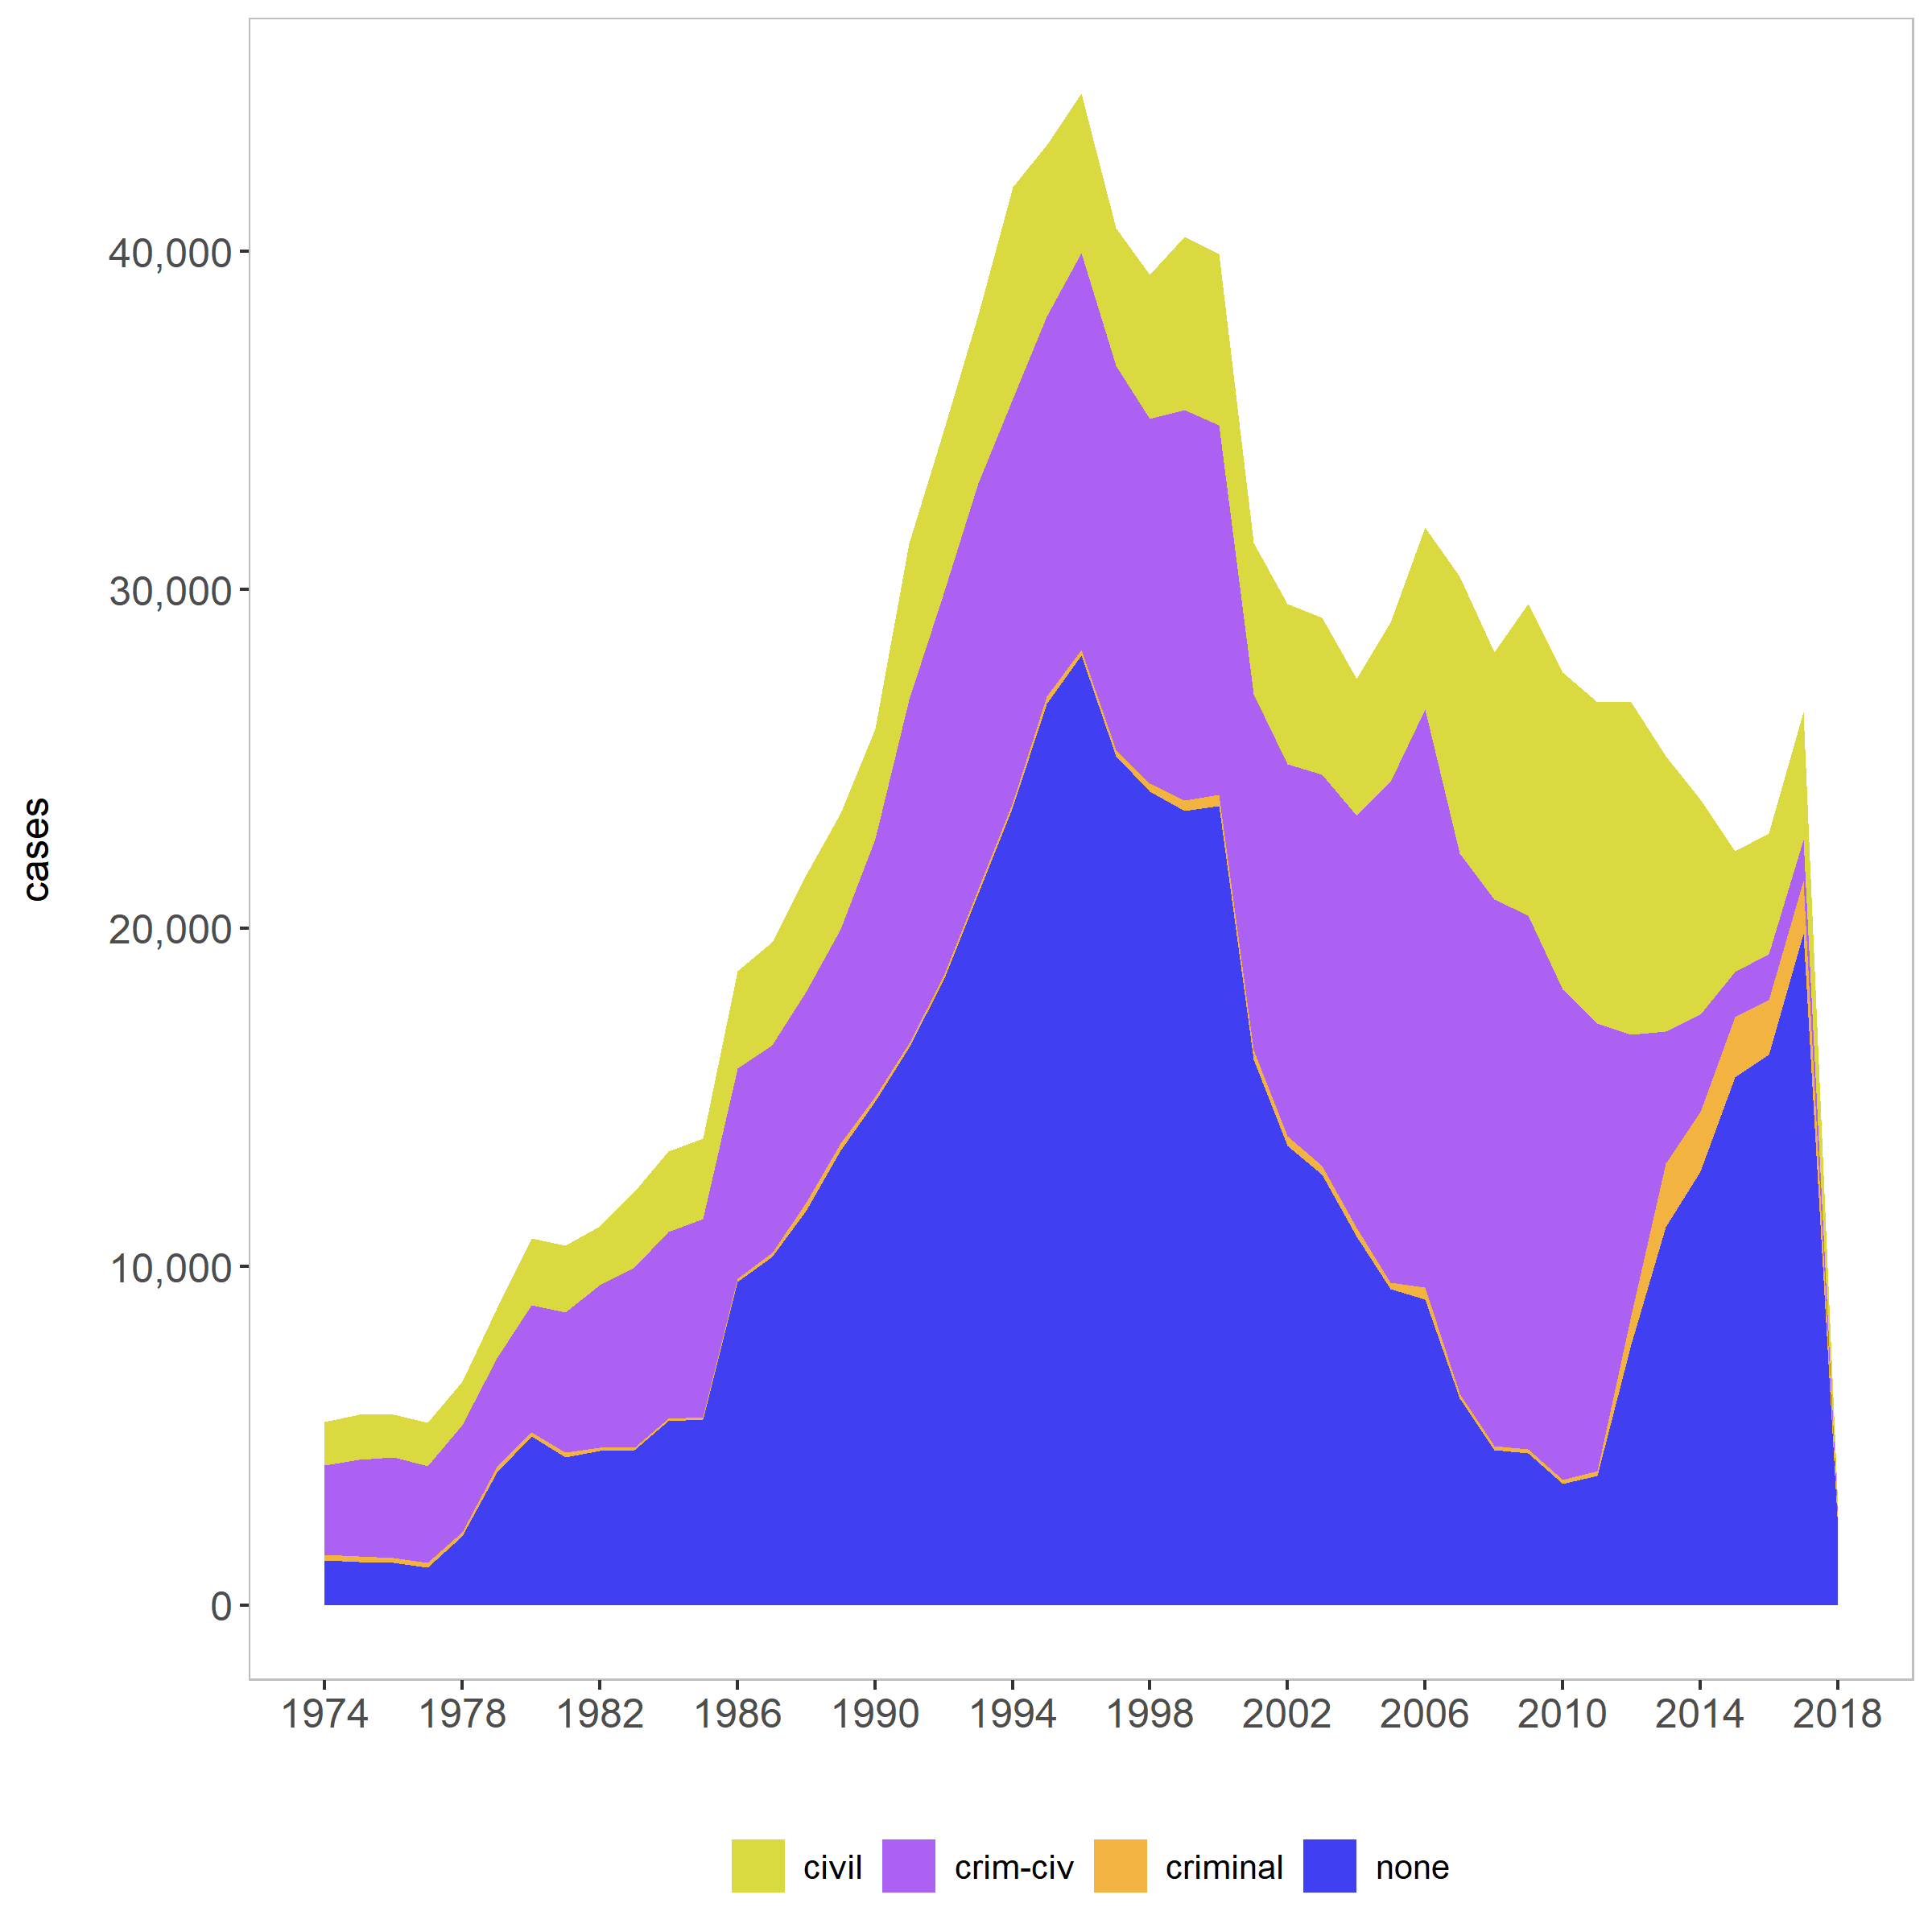
\includegraphics[width=4in]{YearCaseTypeDensity.png}
        \centering
        \caption*{\vspace{-0.5in}}
        \label{}
    \end{figure}
    \normalsize
    \newpage
    
    \item Plot panel of line graphs, cases by court and year:
    \scriptsize
    \begin{verbatim}
        # Aggregate cases by court and year
        x <- dbGetQuery(db,
               "select   year(a.DecisionDate) as Year, b.ShortName, b.LongName, count(1) as n
                from     CaseHeader a left join Court b on a.CourtID=b.ID
                group by year(a.DecisionDate), b.ShortName, b.LongName")
        
        # Convert court col to a factor for face label ordering
        x[,"court"] <- factor(x[,"ShortName"],
                             levels=c("1st Circuit Court of Appeals",
                                      "2nd Circuit Court of Appeals",
                                      "3rd Circuit Court of Appeals",
                                      "4th Circuit Court of Appeals",
                                      "5th Circuit Court of Appeals",
                                      "6th Circuit Court of Appeals",
                                      "6th Circuit Bankruptcy Appellate Panel",
                                      "7th Circuit Court of Appeals",
                                      "8th Circuit Court of Appeals",
                                      "9th Circuit Court of Appeals",
                                      "10th Circuit Court of Appeals",
                                      "11th Circuit Court of Appeals",
                                      "Court of Federal Claims",
                                      "DC Circuit Court of Appeals",
                                      "Federal Circuit Court of Appeals",
                                      "Temporary Emergency Court of Appeals",
                                      "Tennessee Eastern District Court"))

        # Generate line graph, cases by court and year
        ggplot() +
        geom_line(data=x, aes(x=Year, y=n)) +
        scale_x_continuous(breaks=seq(1974, 2018, 6)) +
        scale_y_continuous(label=function(x) format(x, big.mark=",")) +
        facet_wrap(~court, labeller=as_labeller(function(x) sub("rict Court", "",
        sub("Court of ", "",
        sub(" Appellate Panel", "",
        sub(" Court of Appeals", "", x)))))) +
        theme(plot.title=element_text(size=12, hjust=0.5),
        plot.subtitle=element_text(size=10, hjust=0.5),
        plot.caption=element_text(size=10, hjust=0.5),
        panel.background=element_blank(),
        panel.grid.major.x=element_blank(),
        panel.grid.major.y=element_blank(),
        panel.grid.minor=element_blank(),
        panel.border=element_rect(fill=NA, color="gray75"),
        panel.spacing=unit(0, "in"),
        axis.title.x=element_text(size=12),
        axis.title.y=element_text(size=12),
        axis.text.x=element_text(size=10, angle=90, hjust=1, vjust=0.5),
        axis.text.y=element_text(size=10),
        #axis.ticks=element_blank(),
        strip.text=element_text(size=8),
        strip.background=element_blank(),
        legend.position="bottom",
        legend.background=element_rect(color=NA),
        legend.key=element_rect(fill="white"),
        legend.box="horizontal",
        legend.text=element_text(size=10),
        legend.title=element_text(size=10)) +
        labs(x="", y="cases\n")
    \end{verbatim}
    \normalsize
    \newpage
    Result:
    \small
    \begin{figure}[H]
        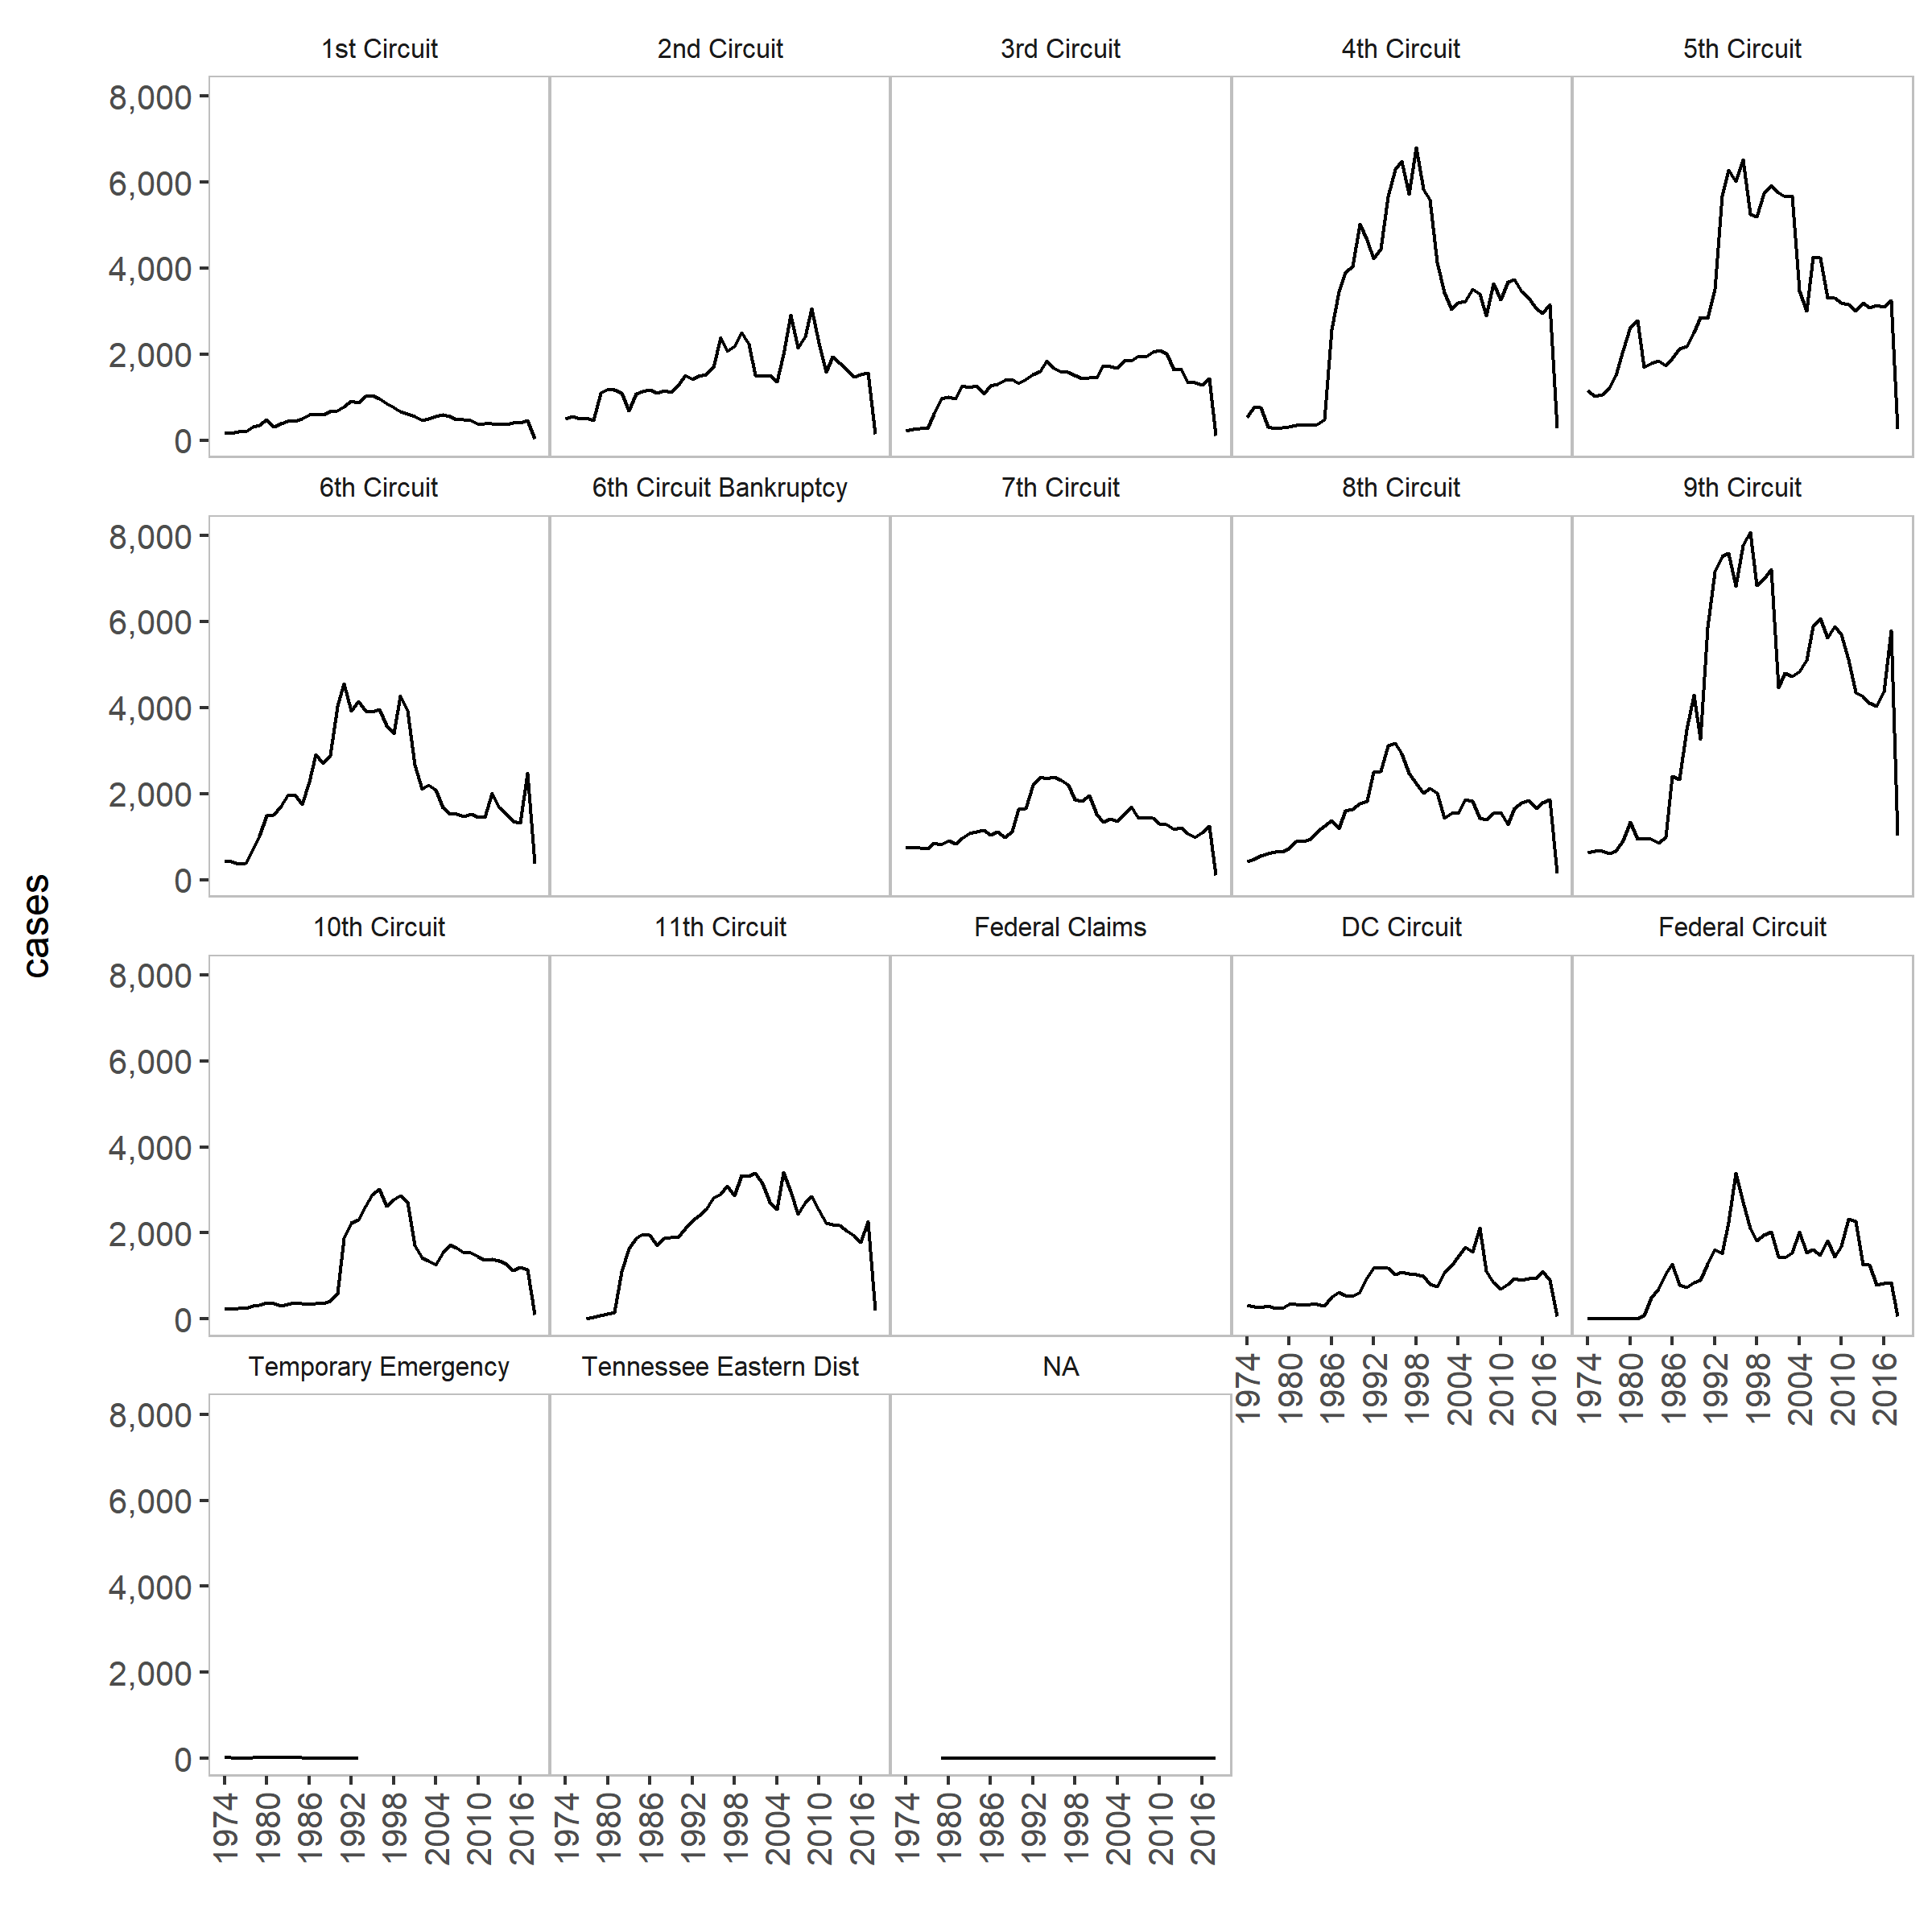
\includegraphics[width=5in]{CourtYearCaseLineGraph.png}
        \centering
        \caption*{\vspace{-0.5in}}
        \label{}
    \end{figure}
    \normalsize


\end{itemize}


\end{spacing}

\end{document} 